\subsubsection{Passo 1: Preparazione}

È importare eseguire una \textit{Business Impact Analisys}, per capire i danni
che ci possono essere al sistema.
Una buona guida può essere porsi le seguenti domande: quando interviene il team
per la gestione dell'incidente? Come possono aiutare le agenzie governative?
Negli USA FBI e in Italia la Polizia Postale.

\paragraph{Tecnologie per il rilevamento}

Ogni organizzazione deve avere le capacità di monitoraggio e di rilevamento
sufficienti per capire se ci sono incidenti, in una misura di tempo ristretta.

\subparagraph*{Decoy} Esiste tutta un'area molto ricca (anche in termini
monetari) che fanno \textit{decoy}, ovvero fanno un falso obiettivo: son sistemi
in uso, account, servizi e altro che sono credibili da parte dell'organizzazione
ma che non sono usabili. Quando vengono usati l'attacco viene rilevato. Questa
metodologia è per certi versi diversa dall'\textit{honeypot} e si diversifica
in quanto è un'operazione per eseguire controlli, non una vulnerabilità fittizia
aperta appositamente.

\subparagraph*{Vulnerabilità e incidenti} Gli incidenti e le vulnerabilità
correlate che vengono registrate tramite i log si stanno rivelando fallimentari
e si sta cominciando ad utilizzare l'intelligenza artificiale come modo per eseguire
analisi su grandi moli di dati.

\paragraph*{Management Participation}

Proporre alternative
\begin{itemize}
\item Include le criticità del business, rischio della proposta, costo e tempo
per il recupero, affidabilità;
\item Costi di ridondanza: preparazione, acquisti di router e computer ridondanti,
capacità di reazione;
\item Costi di detection: NIDS(Network Intrusion Detection System)/HIDS(Host-based
Intrusion Detection System).
\end{itemize}

Il management prende la decisione finale (il senior mngm deve essere convinto
che la soluzione vale i soldi investiti).

\paragraph*{Contenuti IRP}

\begin{itemize}
\item Preparazione preincidente;
\item Come dichiarare il disastro;
\item Procedure di evacuazione;
\item Identificare le persone responsabili, informazioni e contatti.
\end{itemize}

\subsubsection{Passo 2: Identificazione}

\subparagraph*{Triage} Questa operazione (detta anche \textbf{selezione}) si fa
anche negli ospedali (bianco, verde rosso giallo ecc.) e consiste nell'eseguire
una categorizzazione degli eventi. Possibili punti importanti:
\begin{itemize}
\item Che tipo di incidente è avvenuto?
\item Qual è la gravità dell'incidente?
\item Chi dovrebbe essere chiamato?
\item Stabilire una catena di custodia per le prove.
\end{itemize}

È importante che esistano queste tipologie di procedure visto che permettono alla
gente di eseguire in maniera ``automatica'' anche quando ci sono situazioni di
allarme/si è sotto attacco.

\subparagraph*{Catena di custodia delle prove} Un passo che non bisogna fare mai
è inquinare le tracce (anche biologiche) di un indicente. Questo perché
potrebbero essere utili per ricostruire l'incidente e anche per perseguire
chi ha commesso il reato.
In ogni momento l'evidenza deve seguire la catena della custodia.

\subsubsection{Passo 3: Containment}

Si attiva il team di risposta all'incidente per contenere il rischio, si
isola il problema e si ottengono e preservano le prove.

Bisogna anche capire la corretta strategia per contenere i danni. Alcune
soluzioni potrebbero comprendere la disconnessione di rete, ma questo implica
dei costi che vanno valutati.

\paragraph*{Risposta}

Risposta tecnica:
\begin{itemize}
\item Collezionare informazioni sul sistema
\item Analizzare i \textit{log} di sistema
\end{itemize}

Risposta legale: persecuzione legale dell'attaccante. Un problema è
che il personale che si occupa dell'aspetto legale di attacchi informatici è
poco.

\subsubsection{Passo 4: Analisi e Eradicazione}

Determinare com'è avvenuto l'attacco: 5 w del giornalismo. Capire qual è stato
l'impatto e che danni ha causato. Rimuovere la radice per:

\begin{itemize}
\item Ricostruire il sistema;
\item Parlare con l'ISP per ottenere più informazioni;
\item Eseguire un'analisi di vulnerabilità;
\item Migliorare le difese con miglioramenti alle tecniche di protezione.
\end{itemize}

\paragraph*{Analisi}

\begin{itemize}
\item Cos'è successo?
\item Chi è stato coinvolto?
\item Qual è la ragione dell'attacco?
\item Da dove è partito l'attacco?
\item Quando è iniziato l'attacco?
\item Com'è successo?
\item Quale vulnerabilità ha permesso l'attacco?
\end{itemize}


\paragraph*{Rimuovere le radici del problema}

Alcune possibili soluzioni:
\begin{enumerate}
\item Se un account root viene compromesso, non è possibile recuperare per cui è
meglio resettare completamente il sistema formattando tutto e ripristinando i
dati dal backup, sperando che non siano stati compromessi precedentemente;
\item Implementare le patch recenti e gli antivirus, tutte le password devono
essere cambiate.
\end{enumerate}

\subsubsection{Passo 5: Recovery}

Ripristinare le normali operazioni e assicurare che il sistema sia completamente
funzionante e testato.

\subsubsection{Passo 6: Imparare la lezione}

Il follow-up include: scrivere \textit{Incident Report} (che include cosa è andato storto,
quando, quanto è costato, ecc) e presentare il risultato agli stakeholders.

\section{Pianificazione dei processi}
\label{IRBC:pp}

\subsection{Training}

Nel momento in cui subiamo il training diventiamo responsabili. Si distingue tra
colpa (accade sotto la nostra responsabilità) e colpa grave (accade sotto la
nostra responsabilità e siamo tecnicamente preparati per evitare il problema, ma
non l'abbiamo fatto).

\paragraph*{Mentoring} Tipicamente c'è un \textbf{mentor}, ossia qualcuno con
una lunga esperienza che istruisce

\paragraph*{Training formale}

\paragraph*{On-the-job-training} Qualcuno che ti istruisce mentre lavori.


\paragraph*{Penetration Test} Esistono diverse modalità per eseguire dei
penetration test
\begin{itemize}
\item \textbf{External:} test da fuori il perimetro della rete;
\item \textbf{Internal:} test da dentro la rete;
\item \textbf{Blind:} i penetration tester non sanno nulla riguardo a possibili
\textit{decoy} o possibili \textit{honeypot}. Gli amministratori sono a
conoscenza del test;
\item \textbf{Double blind:} come blind, ma anche gli amministratori di sistema non sanno
nulla riguardo l'attacco\footnote{Non è molto utile di solito};
\item \textbf{Targeted:} si hanno informazioni interne sul target. Potrebbe essere
necessario l'accesso ad un account.
\end{itemize}

\subsection{Incident Management Metrics}

\begin{itemize}
\item Numero di incidenti riportati;
\item Numero di incidenti rilevati;
\item Tempo medio di risposta di un incidente;
\item Numero totale di incidenti risolti;
\item Misure prese proattive e preventive;
\item Danno totale degli incidenti riportati e rilevati;
\item Danno totale se gli incidenti non sono stati contenuti per tempo.
\end{itemize}

\subsubsection{Sfide}

Le sfide dell'incident management sono molteplici:
\textit{management buy-in}, \textit{turnover} dell'Incident Management
Team, i problemi di comunicazione e la complessità e la vastità dell'incident response plan.

\paragraph*{Management buy-in}
Il Management non alloca risorse temporali e lavorative per sviluppare
l'incident response plan. Questa soluzione ``a costo zero''
\footnote{Che per la terza legge della termodinamica non può essere mai
zero.} si traduce di norma in un fallimento: alle persone vengono aggiunte
nuove responsabilità e nuovi oneri, che di solito non riescono a portare
a termine.

\paragraph*{Comunicazione} La comunicazione all'interno di un \textit{team} è
importante e non dev'essere né troppa né troppo poca.


\subsection{Esercizi}

Gli esercizi sono disponibili in \ref{esIRBC:pp}

\chapter{Computer Forensics}
\label{IRBC:cf}

\begin{wrapfigure}{r}{0.5\textwidth}
  \begin{center}
    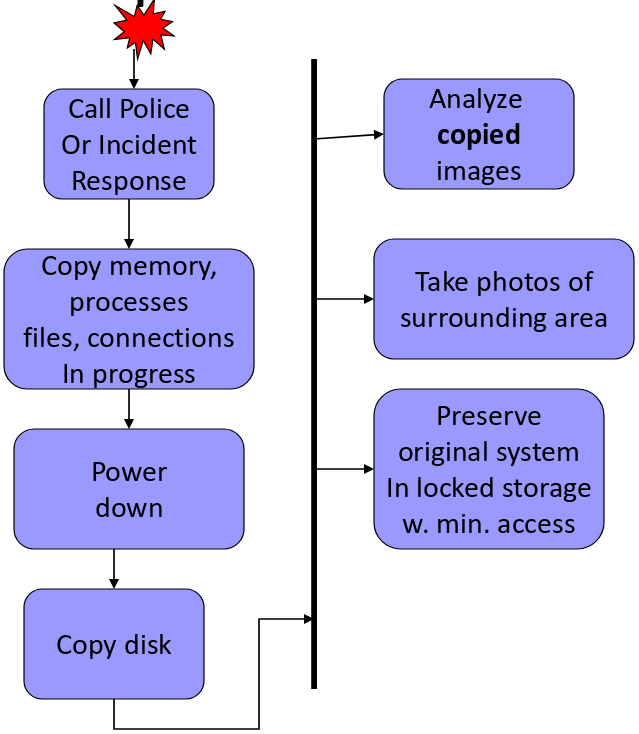
\includegraphics[scale=0.36]{scci}
  \end{center}
  \caption[Passi di una \textit{computer crime investigation}]{
  Questa immagine rappresenta gli \textit{step} da intraprendere dopo
  l'avvenimento di un incidente in un sistema informativo.
  }
\end{wrapfigure}


La \textbf{Computer Forensics} è il processo di identificazione, preservazione,
analisi e presentazione di prove di tipo digitale per un procedimento legale.
Le prove devono rimanere inalterate e la catena di custodia deve essere
mantenuta professionalmente.

Quattro considerazioni principali:

\begin{enumerate}
\item identificare le prove;
\item preservare le prove;
\item analizzare \emph{copie} delle prove;
\item presentare le prove.
\end{enumerate}

Le prove devono passare i test sulla \textbf{autenticità} - la prova è una vera
e affidabile copia della scena del crimine (la computer forensic non distrugge
o altera l'evidenza)- e \textbf{continuità} - la catena di custodia assicura
che la prova sia intatta.

Bisogna tenere conto che le prove devono essere esposte ad avvocati
e quindi è necessario che il lessico usato non sia troppo tecnico e fruibile da tutti.

\section{Preparare una prova}

Lavorare con la polizia per evitare: contaminazione delle prove, liberare la
catena di custodia e infrangere i diritti del sospettato.

Ci sono alcune prove che non possono essere portate in tribunale, a causa di
quella che si chiama \textbf{corrispondenza privilegiata}: sono delle e-mail
di tipo classificato che vengono controllate da un delegato speciale, il quale
conferma o meno se hanno a che fare con il caso. Di conseguenza, è importante
prestare attenzione a come le prove vengono gestite.

\section{Creare una copia forense}

Questo assicura che i contenuti non siano cambiati.
Non si creano delle copie normali ma si effettuano immagini del
disco\footnote{Ad esempio con \texttt{dd} su sistemi Unix}.

La fase di \textbf{indexing} dei dati dev'essere eseguita tramite algoritmi
\textit{smart}, che permette una ricerca più veloce di particolari stringhe di
testo.

\section{Rapporto Legale}

Descrivere i dettagli dell'incidente accuratamente, essere comprensibile e non
ambiguo, offrire valide conclusioni, opinioni o raccomandazioni e descrivere come
le conclusioni sono state raggiunte. Il rapporto deve resistenere ad uno scrutinio
legale, essere creato in maniera rapida e deve essere preciso e facile da essere
riferibile.

\section{Forense}

\subsection{Form della catena di custodia}

Serve a tracciare dove e come le prove sono state gestite; include:
nome e contatto del custode, identificatori dettagliati della prova, quando,
da chi e perché la prova è stata acquisita o spostata, dove viene conservata
e quando/se è tornata.

Inoltre sono presenti log dettagliati delle attività, delle checklist per i
tecnici che la acquisiscono e un form di \textit{non-disclosure} firmato.

\subsection{Log del caso}

Il log del caso include:
\begin{itemize}
\item numero del caso;
\item note basilari, requisiti e procedure del caso;
\item data di quando è stata ricevuta la richiesta;
\item data di assegnazione delle indagini ad un investigatore;
\item data di completamento;
\item nome e informazioni di contatto per l'investigatore e il richiedente.
\end{itemize}

\subsection{Report dell'investigazione}

Include: nome e contatti per l'investigatore, numero del caso, data di
investigazione, dettagli delle interviste o comunicazioni, dei
dispositivi o dei dati acquisiti, dei software utilizzati, dei ritrovamenti
(includendo i dati) e una firma dell'investigatore.

\section{Esercizi}

Gli esercizi sono disponibili in \ref{esIRBC:cf}
